\documentclass[../physical_computing.tex]{subfiles}

\begin{document}

\chapter{Lab Exercise 9 - Commanding the Lights}
\label{sec:appendix_9}

\section{Processor System to Programmable Logic}
\label{sec:ps2pl}

In Appendix \ref{sec:appendix_7} we learned to embed a microblaze processor on an Artix 7 FPGA. The
processor was connected via a UART interface to a terminal window. We used C to write simple programs
that could display things in that window. In this lab we will do several things. First, we will learn
how to use C to detect and store keystrokes from the keyboard connected to the terminal. A sequence of
keystrokes will be stored in memory, until a special keystroke, the `return' key, is detected. Then the 
series of stored keystrokes will be interpreted as a number. Second, we will learn to create a shared
memory between the processor system (PS), the computer we embedded on the FPGA, and the programmable logic
(PL) that we can arrange for ourselves alongside the processor. Finally, we will learn to read out the 
shared memory in programmable logic and display its contents with the LEDs on the BASYS3 board. In both 
the storage of a sequence of characters in memory on the FPGA, and the writing of numbers to shared 
memory, we will need to make use of a facility for direct addressing of memory in C called pointers.
Pointers are the main reason why we choose to use C as opposed to PYTHON or some other higher level
language in this course. 

The structure of this lab will be as follows. First, you should certainly carefully read through the 
notes from the seminar in Week 10. In that class I taught you how to build a terminal program on the 
microblaze processor. We will use that program with very little modification to allow us to send 
numbers that we will type in on the keyboard to shared memory. Second, you will use VIVADO to build
a slightly more complex computer that incorporates a shared memory module and the wiring to connect
the data output of the shared memory to our 16 LEDs. Next you will build the command line interpreter
from Lecture 10 and run it on your modified hardware. The presence of the extra hardware for shared 
memory and LEDs should not prevent the command line interface program from working as I showed you in 
class. Finally, you will add some code to this command line interface so that when you type in a number,
that number is written to shared memory and is mirrored on the LEDs on the BASYS3 board.

\section{Modified Hardware}
\label{sec:modified_hardware}

Figure \ref{fig:afterconnectionautomation} shows the basic hardware configuration that was built in 
Appendix \ref{sec:appendix_7}. We must first add some hardware elements to this block diagram for 
the shared memory facility and the LED outputs. If you have not yet built your embedded system, follow
the instructions in Section \ref{sec:hardware} of Appendix \ref{sec:appendix_7} until you have this 
block diagram built. Now press the '+' button and search for a module called "AXI BRAM Controller".
This is the unit that will interface the shared memory to the bus of the microblaze processor. Once
this block has appeared, double click on it, and reduce the number of AXI BRAM interfaces from the 
default of 2 to 1. Next, add a second hardware element called "Block Memory Generator". Once this block
has appeared, double click on it too, and alter it to "True Dual Port RAM". Also check the small box 
for "Common Clock". Now click on 'run connection automation' and select 'all automation' to wire the
shared memory into the rest of the hardware.

On the left hand side of the Block Memory Generator, you should see that one of the two BRAM ports is
wired to the AXI BRAM Controller, but the other one is unwired. If you click on the '+' sign next to
this unwired controller, it will expand to reveal 7 ports. We will need to connect all of these up to
use the shared memory. Sometimes an unused port may disappear from the GUI interface. If this happens,
close and reopen the expansion by clicking on '-' then '+' again, and the port should reappear. The 
first and easiest wire is the reset port, labelled 'rstb'. Wire this to 'reset' on the left hand side of the diagram.
Next, we need to wire up the clock input, labelled 'clkb'. I have found it best to create a dedicated clock 
port to wire this to. To do this, double click on the 'Clocking Wizard' module, select the 'Output Clocks' tab
and check the second unused output, then click OK. A clock output port should appear, and you should wire this to 
'clkb' on the Block Memory Generator. 

There are several ports on the Block Memory Generator that need constant inputs of various descriptions. 
These are labelled 'addrb', 'dinb', 'enb' and 'web'. The simplest of these is 'enb', which is  a simple
enable line, and should be set to '1'. To do this, use '+' and search for 'Constant'. When this block 
appears, wire the output to 'enb'. The default output for 'Constant' is a single bit with value 1, so you
don't need to change anything. Now get another 'Constant', but this time double click on it, and change
its data so its Width is 32 bits and its value is 0. This one should be wired to both 'addrb' and 'dinb'. 
The 'addrb' allows you to select the starting byte in the address space of the shared memory for the data
we will be reading. Since we will simply use the very first byte of the address space, this offset is set
to zero. The 'dinb' bus allows you to write to shared memory from programmable logic. We won't be doing 
this, so we just set this input to zero as well. We use the same 32 bit wide zero to wire to both inputs
to save space in the diagram. The 'web' input enables on-the-fly reconfiguration of shared memory, but we
won't need this, so this needs to be connected to another constant, equal to zero, four bits wide. Connect
that one up as well. 

Next to connect the output data. Note that this is 32 bits wide, but we only have 16 LEDs. We shall use these
LEDs to display the contents of the lowest 16 bits of the data in the first 32 bit space of addresses in the 
shared memory. To access the lowest 16 bits of a 32 bit field, we import a block called 'Slice'. This block
should be moved to under the Block Memory Generator. Double click on it and set 'Din from' to 15 and 'Din Down To'
to 0. 'Dout Width' should automatically adjust to 16. Wire the input of Slice to the doutb output of the Block
Memory Generator'. 

Next, we need to connect up the LEDs. You'll need to add a constraint file to the Vivado project. Use the 
fully commented constraint file as usual, and only uncomment the 16 LEDs. Now right click on the Dout output of
Slice, and select 'Make External'. The port name will be Dout\_0 by default. Click on it, and in a window to the left
of the GUI, a box next to Name should say Dout\_0. Click in this box and change the name to led, and hit return. 
The port name should change to 'led'. Now press the button at the top of the gui window with the circle-arrow in 
it to reorganise the diagram. It should now look like the one in Figure \ref{fig:sharedmemoryhardware}. Click on the 
box with a tick in it and let Vivado run a hardware check on your diagram as a rudimentary check that you haven't  
left anything critical out or left any loose wires hanging around.

\begin{sidewaysfigure}
\centering
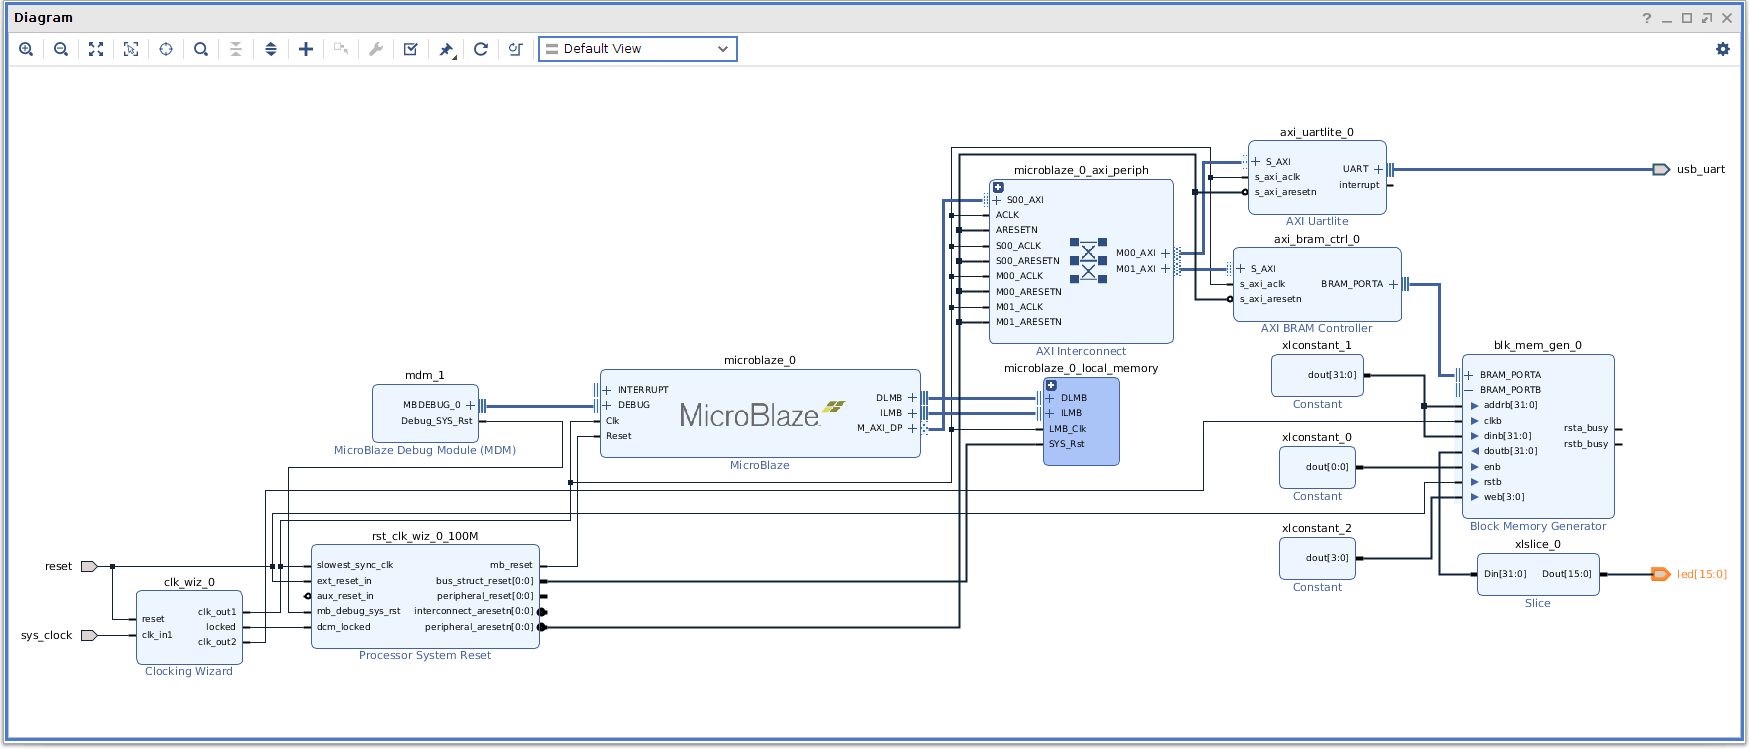
\includegraphics[width=18cm]{appendix_10/figures/sharedmemoryhardware.png}
\caption{Hardware for the shared memory project}
\label{fig:sharedmemoryhardware}
\end{sidewaysfigure}

If you have not already done so, create an HDL wrapper for your hardware using the instructions in Section 
\ref{sec:hardwarebuild}. You should now be able to carry on following the instructions in this section to 
run synthesis, run implementation and generate the bitstream. Just continue with the instructions until you 
have exported the project. One interesting aspect is to look at a tab that should have appeared in the main 
project pane in Vivado called 'Address editor'. This shows a rough memory map of the address space of buses
connected to the microblaze processor. Notice that axi\_bram\_ctrl\_0 occupies address \texttt{0xC0000000}. We
will encounter this address again when we write the code.

\section{Software for the Light Controller}
\label{sec:lightcontrolsoftware}

The software can mostly be re-used from the terminal program that was developed for Seminar 6. See page 14 of
the notes from this seminar. The program is reproduced below. You will need to go through the notes of the seminar
to make sure you understand the use of pointers/addresses to write data to memory and read it back. 

\begin{minted}{c}
#define CMD_BUF_LEN 20
int main()
{
  u32 charcount;
  unsigned char inp;
  char cmdbuffer[CMD_BUF_LEN];
   while(1) {
    xil_printf("\r\n$ ");
    charcount=0;
    while(charcount<CMD_BUF_LEN) {
       xil_printf("\r\n$ ");
	  charcount=0;
	  while(charcount<CMD_BUF_LEN) {
		inp=XUartLite_RecvByte(XPAR_UARTLITE_0_BASEADDR);
		if(inp!=(unsigned char)'\r') {
		  xil_printf("%c",(char)inp);
		  cmdbuffer[charcount]=(char)inp;
		  ++charcount;
		} else {
		  cmdbuffer[charcount]='\0';
		  xil_printf("\r\nCompleted command was %s",cmdbuffer);
		  charcount=CMD_BUF_LEN;
		}
	  }
	  if(inp!='\r') {
		  xil_printf("\r\nERROR: command buffer full");
	  }
	}
    return;
}
\end{minted}

The key statement allowing the detection and ingestion of keystrokes from the terminal keyboard is
\texttt{inp=XUartLite\_RecvByte(XPAR\_UARTLITE\_0\_BASEADDR)}. This is a call to wait for a key press
on the keyboard, and load the character corresponding to that key into the variable \texttt{inp}, which
is of the somewhat obscure data type \texttt{unsigned char}. This character data is written to a 
memory address, or pointer \texttt{cmdbuffer+charcount}. The variable \texttt{charcount} is incremented
each time a character is stored, so that the sequence of keystrokes ends up in an array. Once the
return key is hit, the termination character is appended to the end of the character array.
Currently in the code nothing is done with the character string.

You should open Vitis, select the base address of your project as the working directory, and following the 
instructions in Appendix \ref{sec:appendix_7} import the hardware file, which is a file called
\texttt{<project name>.xsa}, into the IDE. Start a new hello world project as we did before, but now replace
the code in \texttt{hello\_world.c} with the above code for the terminal emulator, ensuring that you also 
have the correct set of include files, given on page 13 of the notes from seminar 6:

\begin{minted}{c}
#include <stdio.h>
#include <stdlib.h>
#include <string.h>
#include "xil_types.h"
#include "xparameters.h"
#include "xuartlite.h"
\end{minted}

After saving the modified source code you should build the project, start the terminal, configure the terminal
following the instructions in Section \ref{sec:helloworld}, and run the code, checking that the terminal prompt
appears in the terminal window, and that you can enter commands up to 20 characters long. After you press return, 
the command should be echoed back to you on the terminal, and if you exceed 20 characters this should be detected
and induce an error. It's a simple, decently robust, terminal, but it has no interpreter.

\section{The simplest possible interpreter}
\label{sec:simpleinterpreter}

We wish in the simplest possible way to interpret this character string as an unsigned integer, and to write this
integer to shared memory so that its value can be displayed with the LEDs. First we will need a variable of an 
appropriate type whose location is the address of the shared memory. The address we require is 
\texttt{0xC0000000} which if you recall was in the memory map in hardware. We could hard code this address, 
but this isn't a very robust approach. Better than that, it turns out that the header file \texttt{xparameters.h}
defines a preprocessor string which corresponds to this address. Were we to alter our hardware, and the base
address of the shared memory were to change, the file \texttt{xparameters.h} would be altered to contain the 
modified base address, and there would be no need to update our C code. Using the Explorer pane in IDE, open
the folder labelled \texttt{design\_1\_wrapper}. Navigate to \texttt{xparameters.h}, which is at the path shown
below. Line 552 of this file contains the \texttt{\#define} for a preprocessor variable \texttt{XPAR\_BRAM\_0\_BASEADDR}
to the required address in the memory map.

\begin{minted}{shell}
microblaze_0/standalone_domain/bsp/ \
microblaze_0/include/xparameters.h
\end{minted}

Note that when you open this file in the IDE the contents are displayed in a new tab, but the source you are
modifying has not disappeared, and is in another tab behind which you can return to and carry on coding.
To associate this particular address with a 16 bit variable, insert the following variable declaration
immediately following the opening curly brace of the main program.

\begin{minted}{c}
u16 *pled=XPAR_BRAM_0_BASEADDR;
\end{minted}

The next task is to insert a line of code that interprets the input keystrokes as a number. A simple way of 
doing this is to use the \texttt{atoi} function built in to C, which essentially takes a character string and
attempts to interpret it as an integer. This integer is then cast to an unsigned short integer of the 
xilinx inbuilt type \texttt{u16}, and this number is stored at the memory location that is mapped to the shared
memory in hardware. On the other, programmable logic side of the fence, the data at this memory location is 
wired to the LEDs. The line you need to alter in the C code is the line where the command was echoed back to you, 
which currently as follows.

\begin{minted}{c}
xil_printf("\r\nCompleted command was %s",cmdbuffer);
\end{minted}

Replace this command with the following invocation of \texttt{atoi}.

\begin{minted}{c}
*pled=(u16)atoi(cmdbuffer);
\end{minted}

This command interprets the string of characters at the address \texttt{cmdbuffer} as an integer, and
then casts that integer into data type \texttt{u16}, storing the result at the address pled, which is
\texttt{0x0000000C} in the memory map, the memory location shared with the programmable logic.

Recompile your code and after recompiling, you should see that numbers you typed in are displayed in 
binary on the 16 LEDs. An additional nice feature is that if you type in anything that is less than 
20 digits long but isn't a number, the behaviour of \texttt{atoi()} is to return zero. So, none of the
LEDs light up. This is a reasonable, though not very revealing, failure mode.

\section{Coding challenges}
\label{sec:codechallenge}

Here are some other projects that you might try to enhance the terminal based LED controller.

First, you could use the driver you previously built for the 4 character 7 segment display to 
display the number you enter in hexadecimal on the LED display instead. This is a matter of 
creating a graphical 'IP' from your LED controller, making the exported control visible to 
your graphical designer in Vivado, adding the controller to the hardware, connecting it to the
clock (you'll need to create a further clocking wizard output to connect it), modifying the 
constraint file so that the LED ports are available on the diagram, and wire the input to your
LED display driver to the \texttt{doutb} port on the shared memory. Make the outputs of your 
LED display driver external, and change the names of the external ports to match their names in 
the constraint file. You will need to rebuild your hardware, and re-export it to your project directory.
Vitis will almost certainly spot that the \texttt{xsa} file has been updated, and ask you whether 
you want to update the software project. You will then need to rebuild everything in VITIS, both
the \texttt{design\_1\_wrapper} folder and and the application folder (highlight the directory 
and then hit the hammer button in each case. Re-launch your bitstream in Vivado onto the BASYS3
and run the Vitis project.

Secondly, notice that in hardware we dumped the upper 16 bits of the 32 bits of shared memory. We
could instead wire these upper 16 bits to the 4 digit display, whilst keeping the lower 16 bits
connected to the LEDs. Now you will need software that can set the value of either of these 16 bits
of shared memory. In C code, you can make use of pointer arithmetic. For example, to set the values
of the unsigned shorts in the two 16 bit memory segments, we could do

\begin{minted}{c}
*pled=3;
*(pled+1)=7;
\end{minted}

which sets the lower 16 bits to contain 3, and the upper 16 bits to contain 7. However, you will 
also need a slightly more sophisticated controller in C so that you can type in a number and have
your software know whether you want it to appear on the display or the LEDs. You can either cheat
or do it properly. I would cheat first. Exploit the fact that integers can be negative, and put 
something like this in your C code:

\begin{minted}{c}
/* declaration at the top of main */
int posneg;

/* in the body of the code */
if(posneg<0) {
  *pled=(u16)(-posneg);
  } else {
  *(pled+1)=(u16)posneg;
  }
\end{minted}

Following appropriate modifications to the hardware to connect the upper 16 bits to the display, 
this hack effectively allows you to use negative inputs to set the LEDs and positive inputs to set the
display. It is, however, not very user friendly - who ordered the sign of numbers dictating where
they end up? You may want instead to do it more properly. In this case, you need actual commands and a
primitive interpreter for those commands. You'd like to be able to enter `leds=value' and have the
LEDs display the value, or `display=value' and have the LEDs display the same thing. In this case
you need to analyse the entered string for the occurrence of the '=' symbol. Everything before this 
symbol is interpreted as the command, and everything after this symbol is interpreted as the value. 

A command for finding a particular character in a string in C is \texttt{strstr()}, which returns a
pointer to the start of the first occurrence of that character or character sequence.
If \texttt{strstr} can't find the character or sequence at all, it
returns \texttt{NULL}. You replace the value at the pointer to the equals sign with the string termination 
character, and run atoi on an address one past this inserted termination character, to cast the remainder
of the string as an integer. You then read the command, which is the portion of the string at the 
address \texttt{cmdbuffer} before the newly inserted termination character, as a command, and see whether
it contains the sequence led. If it does, you write the value to \texttt{*pled+1}, and if it doesn't you write
value to \texttt{*pled}.

\begin{minted}{c}
/* at the top */
char* pvalue;
/* in the body, find the equals sign */
pvalue=strstr(cmdbuffer,'=');
/* replace the equals with a string termination */
*(pvalue)='\0';
/* read the command and act accordingly, using atoi */
/* to interpret the characters at the address following */
/* the newly inserted termination as a number, casting */
/* it to u16 and writing to the appropriate shared */
/* memory location */
if(strstr(cmdbuffer,"led")!=NULL) {
  *(pled+1)=(u16)atoi(pvalue+1);
  } else {
  *(pled)=(u16)atoi(pvalue+1);
  }
\end{minted}

A final comment on this code. I have completely abandoned making it robust to syntax errors. What does the
code do if there is no equals sign in the string? Probably something undesirable. Also, any command that doesn't
contain the character sequence led is interpreted as a directive to send the data to the display. If there was
some third command, this would not work. You might want to error
trap the return value of null into pvalue so that nonsense entries are dealt with robustly in the code, and
further error trap the scenario where the command doesn't contain led or display.
Having done that, congratulations you've written your first (very primative) command line interpreter on
an embedded system!

\end{document}